% ----- Bad Instance -----

\subsection{Bad Instance}

As we have seen when choosing our criteria, although our algorithm works very well in general, some instances may be more advantageous on other criteria. So there are instances where our algorithm will not be the best. 
\bigskip

Our algorithm takes the highest degree vertex, so a bad instance would be when the highest degree vertex is not part of the MEWC. 
\bigskip

Also, since we generated the graphs randomly, we usually get a consistent result. But if we are in a case with very heterogeneous values it can happen to have results very far from the MEWC. Here in figure \ref{fig:bad-instance-vertex-highest-degree1}, the MEWC includes a vertex that is not reachable with this choice.

\begin{center}
    \begin{figure}[H]
        \centering
        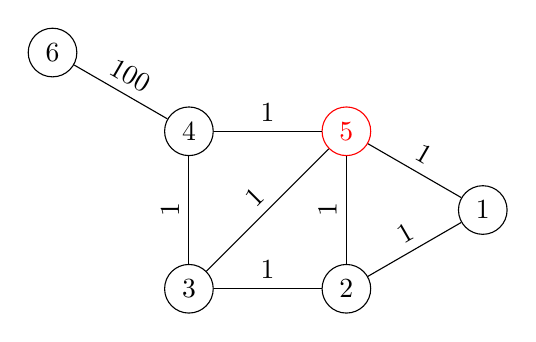
\begin{tikzpicture}[node distance=2cm]
            \node[circle, draw] (1) {1};
            \node[circle, draw] (2) at ([shift=(210:2)] 1) {2};
            \node[circle, draw] (3) [left of=2] {3};
            \node[circle, draw] (4) [above of=3] {4};
            \node[circle, draw, red] (5) [above of=2] {5};
            \node[circle, draw] (6) at ([shift=(150:2)] 4) {6};

            \draw  (1) -- (2) node[midway, above, sloped] {1};
            \draw (1) -- (5) node[midway, above, sloped] {1};
            \draw (2) -- (3) node[midway, above, sloped] {1};
            \draw (2) -- (5) node[midway, above, sloped] {1};
            \draw (3) -- (4) node[midway, above, sloped] {1};
            \draw (4) -- (5) node[midway, above, sloped] {1};
            \draw (4) -- (6) node[midway, above, sloped] {100};
            \draw (5) -- (3) node[midway, above, sloped] {1};
        \end{tikzpicture}
        \caption{Graph illustration for bad instance of our algorithm when we choose the highest degree vertex as criteria 1}
        \label{fig:bad-instance-vertex-highest-degree1}
    \end{figure}
\end{center}

Moreover, our algorithm takes the highest degree vertex to add a new vertex to the solution S. This raises the same problems as those presented by the criterion. The algorithm can form a clique with a vertex that does not belong to the MEWC or is worse while the initial clique could be part of the MEWC or a better solution. Here in figure \ref{fig:bad-instance-vertex-highest-degree2}, the algorithm will take 5 $\rightarrow$ 2 $\rightarrow$ 3 when every other choice could lead to a better clique. 

\begin{center}
    \begin{figure}[H]
        \centering
        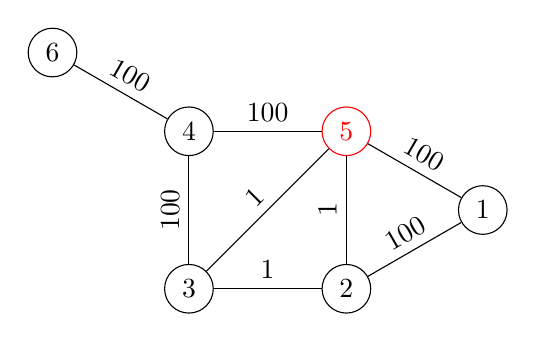
\begin{tikzpicture}[node distance=2cm]
            \node[circle, draw] (1) {1};
            \node[circle, draw] (2) at ([shift=(210:2)] 1) {2};
            \node[circle, draw] (3) [left of=2] {3};
            \node[circle, draw] (4) [above of=3] {4};
            \node[circle, draw, red] (5) [above of=2] {5};
            \node[circle, draw] (6) at ([shift=(150:2)] 4) {6};

            \draw  (1) -- (2) node[midway, above, sloped] {100};
            \draw (1) -- (5) node[midway, above, sloped] {100};
            \draw (2) -- (3) node[midway, above, sloped] {1};
            \draw (2) -- (5) node[midway, above, sloped] {1};
            \draw (3) -- (4) node[midway, above, sloped] {100};
            \draw (4) -- (5) node[midway, above, sloped] {100};
            \draw (4) -- (6) node[midway, above, sloped] {100};
            \draw (5) -- (3) node[midway, above, sloped] {1};
        \end{tikzpicture}
        \caption{Graph illustration for bad instance of our algorithm when we choose the highest degree vertex as criteria 2}
        \label{fig:bad-instance-vertex-highest-degree2}
    \end{figure}
\end{center}